\clearpage
\section{Supplementary material}
\label{sec:4_supplement}
\renewcommand{\thefigure}{S\arabic{figure}}
\setcounter{figure}{0}    

% Figure 4.S1 (ROIS)
% ------------------
\begin{figure}[!tbh]
    \centering
    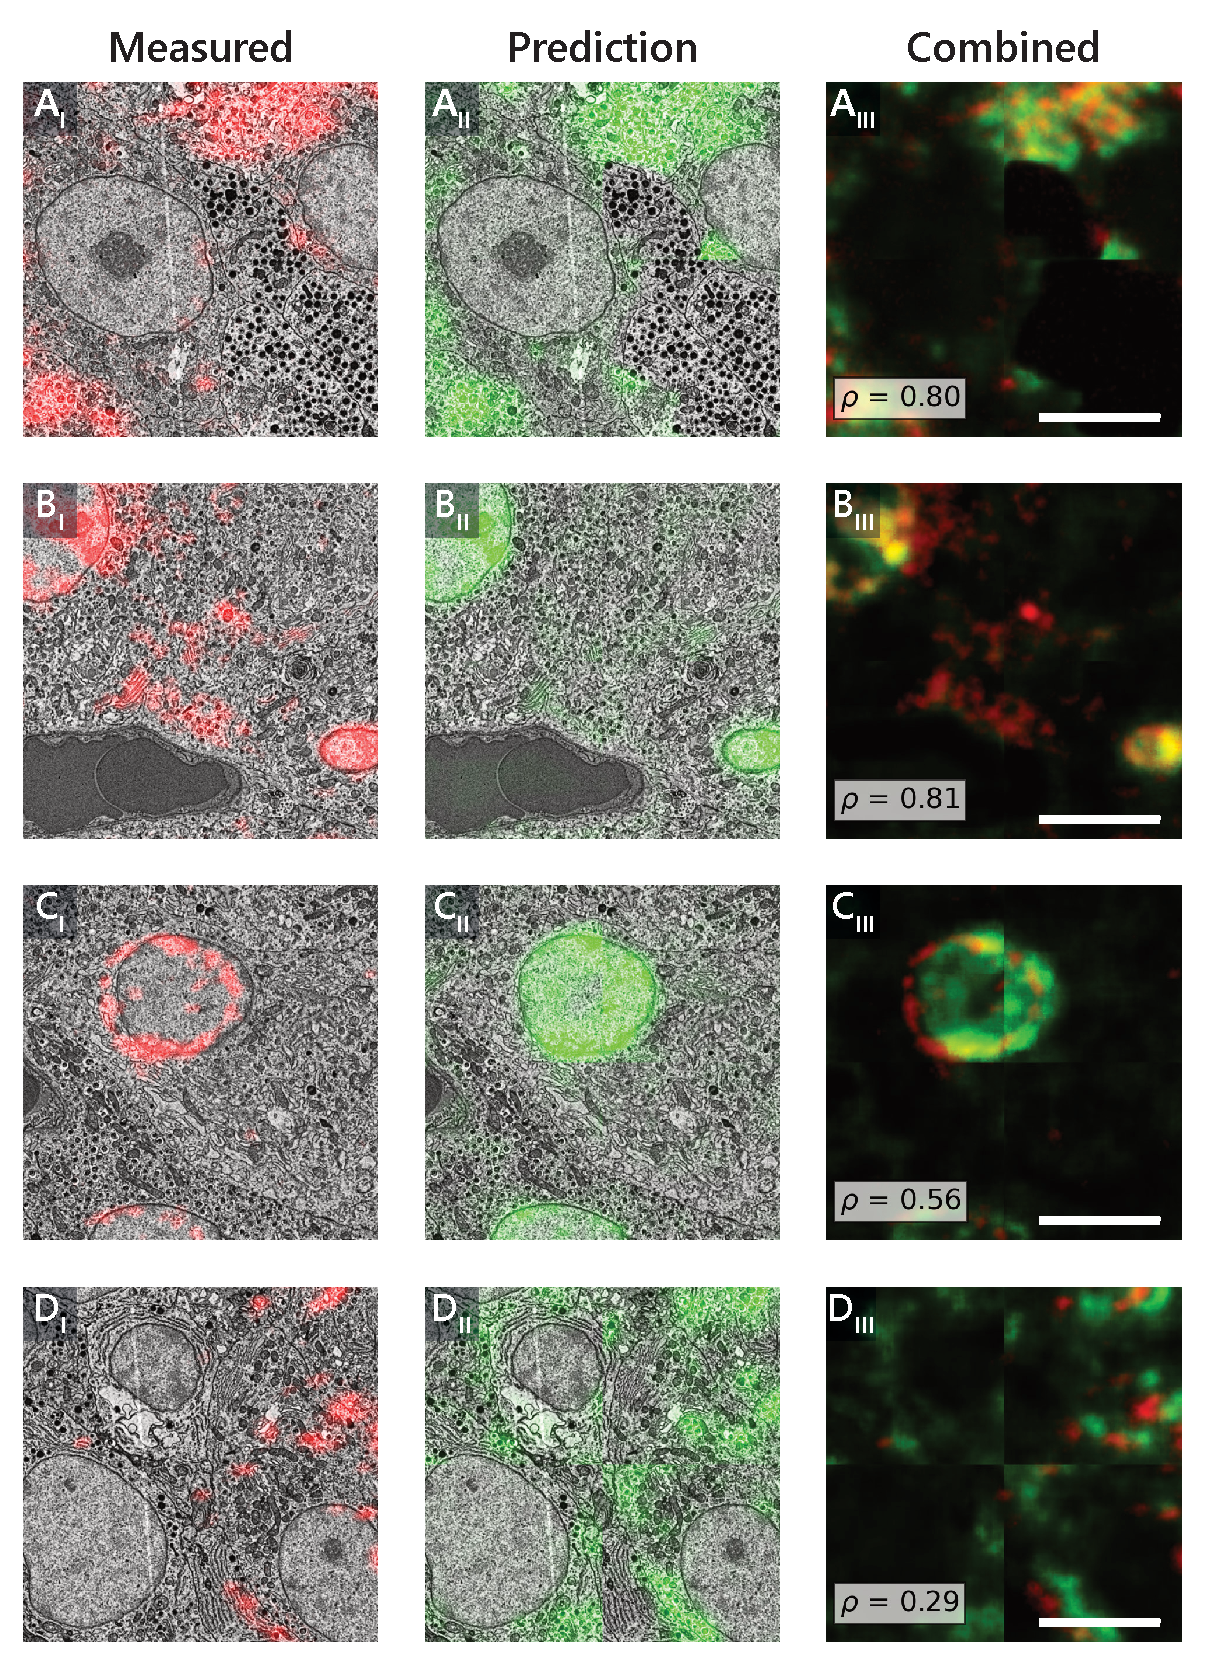
\includegraphics[width=0.95\linewidth]{chapter-4/figures_PDF/fig4-S1_rois.pdf}
    \caption{CLEMnet is able to perform nontrivial structural recognition tasks as well as mitigate issues inherent to fluorescence imaging. (Continued on next page\ldots)}
    \label{fig:4.S1_rois}
\end{figure}
\addtocounter{figure}{-1}
\begin{figure}
    \caption{For each selected ROI (A-D), the measured fluorescence (left, red) and prediction (center, green) are overlaid onto the EM, and combined to show overlap and differences in signal intensity (right).
    (A) The network is able to distinguish between insulin and similar-looking glucagon granules, a difficult task for non-experts.
    (B) An instance of AF594 emission from \SI{405}{\nano\meter} Hoechst excitation demonstrates that the network prediction is less susceptible to bleedthrough. 
    (C) As the network generates predictions directly on structures within the EM, it is able to compensate for errors in the EM-FM registration near the edges of the field of view where the registration may be extrapolated.
    (D) The network is for the same reason also less susceptible to off-axis aberrations such as vignetting, which results in diminished signal at the corners of the fluorescence field of view.
    Note that several predictions are stitched together to compose the predicted image shown, at times giving rise to edge artefacts.
    Scale bars: (A--D) \SI{5}{\micro\meter}.}
\end{figure}

\quad
